\section{Grundlagen}

	\subsection{Eingabegeräte für Schwerstmehrfachbehinderte}
    \label{sec:input-devices}
    
    	Aufgrund der Vielzahl an möglichen Behinderungen und Einschränkungen gibt es eine mindestens genau so große Zahl an Eingabemethoden und Geräten. Diese Eingabegeräte können sowohl eine Schnitstelle zu klassischen PC's darstellen oder auch zur Bedienung von unterstützenden Technologien wie z. B. eines Rollstuhls benutzt werden. Im folgenden sollen hier exemplarisch einige solcher Eingabegeräte vorgestellt werden. Die hier vorgestellte Auswahl ist nicht vollständig und ist aus den Onlinekatalogen der \emph{RehaMedia GmbH} und der \emph{REHAVISTA GmbH} sowie den Webseiten der erwähnten Hersteller zusammengetragen.
        
        \subsubsection*{Augensteuerung}
        	Hierbei werden mit Hilfe einer Kamera die Bewegungen der Augen genutzt um ein Gerät zu steuern. Damit können dann auch Windows oder OS X Betriebssysteme gesteuert werden. Der Anbieter \emph{RehaMedia} bewirbt das System \emph{Tobii PCEye} mit den Worten: \enquote{Die Augensteuerung erfasst die Augenbewegungen und setzt sie präzise in Mausbewegungen um. Dank eines Mauszeigermenüs stehen auch bei der Bedienung mit der Augensteuerung alle Mausfunktionen wie Doppelklick, Rechtsklick usw. zur Verfügung.} \parencite{Rehamedia:TobiiPCEyeGo}
            
         \subsubsection*{Taster}
         	In der Regel handelt es sich bei Tastern um einen einzelnen großen runden Knopf (\autoref{fig:bigRed}). Es gibt aber auch andere ausführungen wie einen Griff, welchen man zusammendrücken kann oder einen befestigten Stab gegen den man Druck ausüben kann. Manche Taster können auch an der Kleidung oder an einer Kopfstütze angebracht werden, so dass eine Bedienung nicht nur mit den Händen sondern auch mit dem Kopf oder durch zusammenschlagen der Knie möglich ist. Pedale zur Bedienung mit den Füßen werden auch angeboten. Die meisten Taster verwenden einen 3,5 mm Klinkenstecker und können damit Signale senden. Der Hersteller \emph{ablenet} bietet z. B. Spielsachen an, die so gesteuert werden können (\autoref{fig:penguinRace}). Andere Eingabegeräte können auch Anschlüsse für diese Taster bereitstellen so das diese kombiniert werden können.  
         	
            \begin{figure}[H]
				\centering
				\begin{subfigure}{.5\textwidth}
  					\centering
  					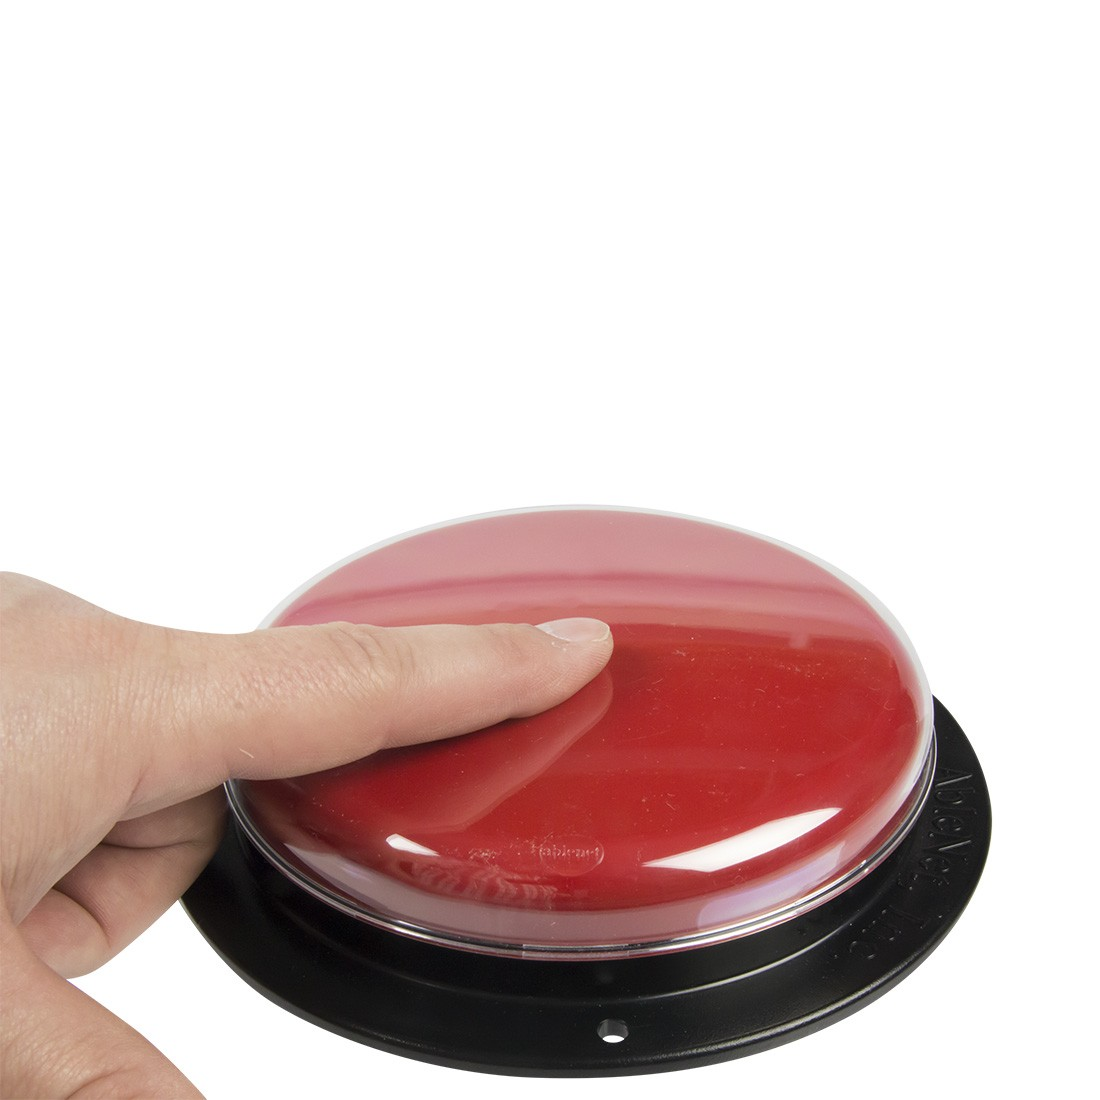
\includegraphics[width=.8\linewidth]{images/big-red-button.jpg}
  					\caption{\emph{Big Red} \cite{ablenet:bigRed}}
                    
  					\label{fig:bigRed}
				\end{subfigure}%
				\begin{subfigure}{.5\textwidth}
  					\centering
  					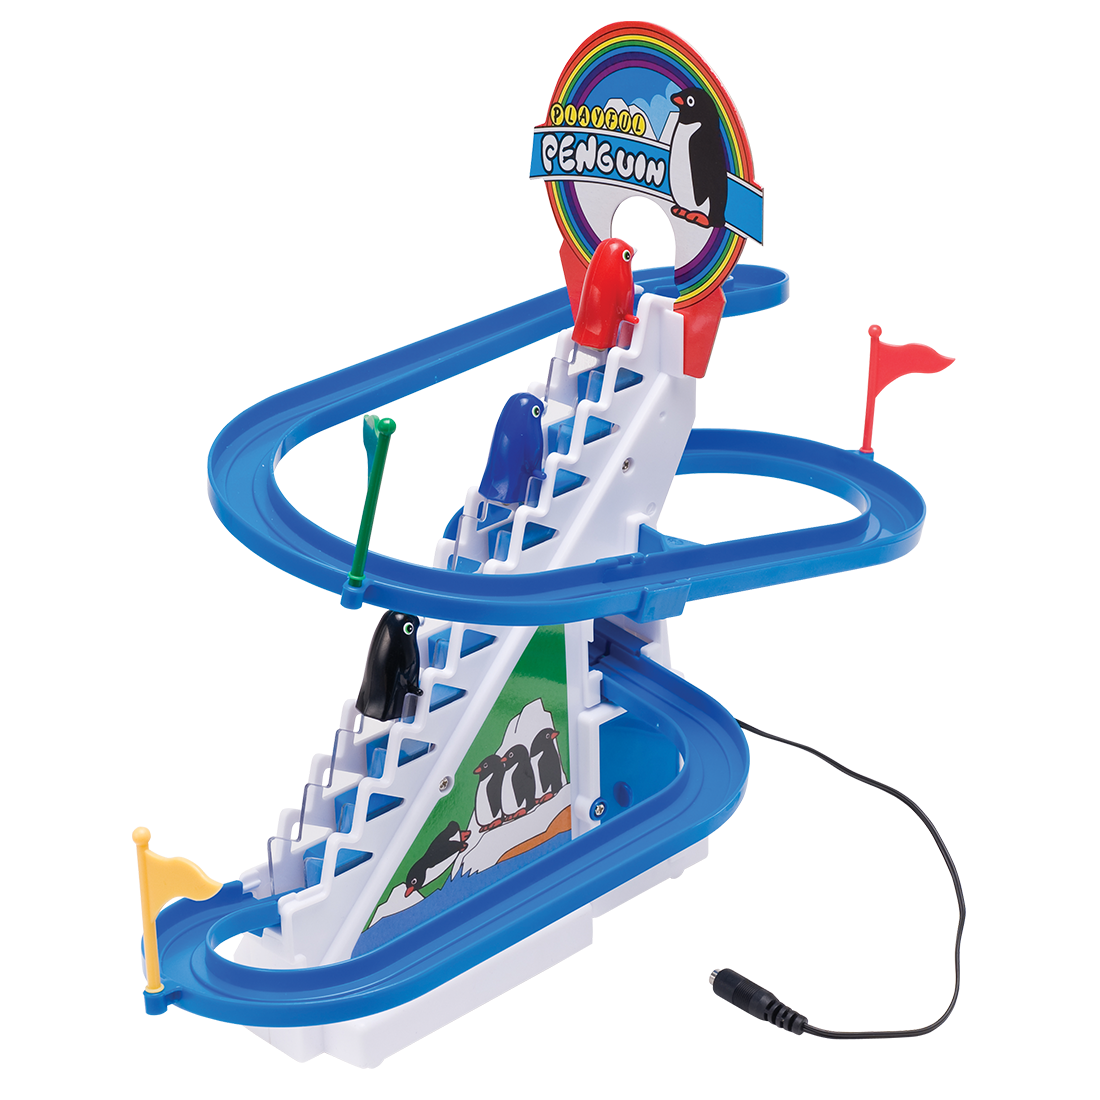
\includegraphics[width=.8\linewidth]{images/penguin-race.png}
  					\caption{\emph{Penguin Race} \cite{ablenet:penguinRace}}
  					\label{fig:penguinRace}
				\end{subfigure}
                \caption{Taster und Spielzeug von ablenet}
				\label{fig:ablenetSingleButtons}
			\end{figure}
            
            Eine weitere Ausführung sind \emph{sprechende Tasten}. Diese Taster haben einen Lautsprecher eingebaut und bieten die Möglichkeit eine oder mehrere Sprachnachrichten aufzunehmen. Wenn mehrere Nachrichten aufgenommen werden können, kann die auszugebende Nachricht von einer betreuenden Person voreingestellt werden. Andere Geräte funktionieren nach dem Prinzip: einmal drücken gibt Nachricht Nummer eins aus, zweimal Nachricht Nummer zwei und dreimal Nachricht Nummer drei.
            
        	Außerdem gibt es Taster mit mehr als einer Taste. Diese sind dann schon zum Anschluss an Computer oder Tablets gedacht und haben häufig einen \emph{USB} oder \emph{Bluetooth} Anschluss. Der Tastenumfang geht dabei von einfachen Geräten mit zwei Tasten bis zu kompletten Computertastaturen.
            
            \begin{figure}[H]
				\centering
				\begin{subfigure}{.33\textwidth}
  					\centering
  					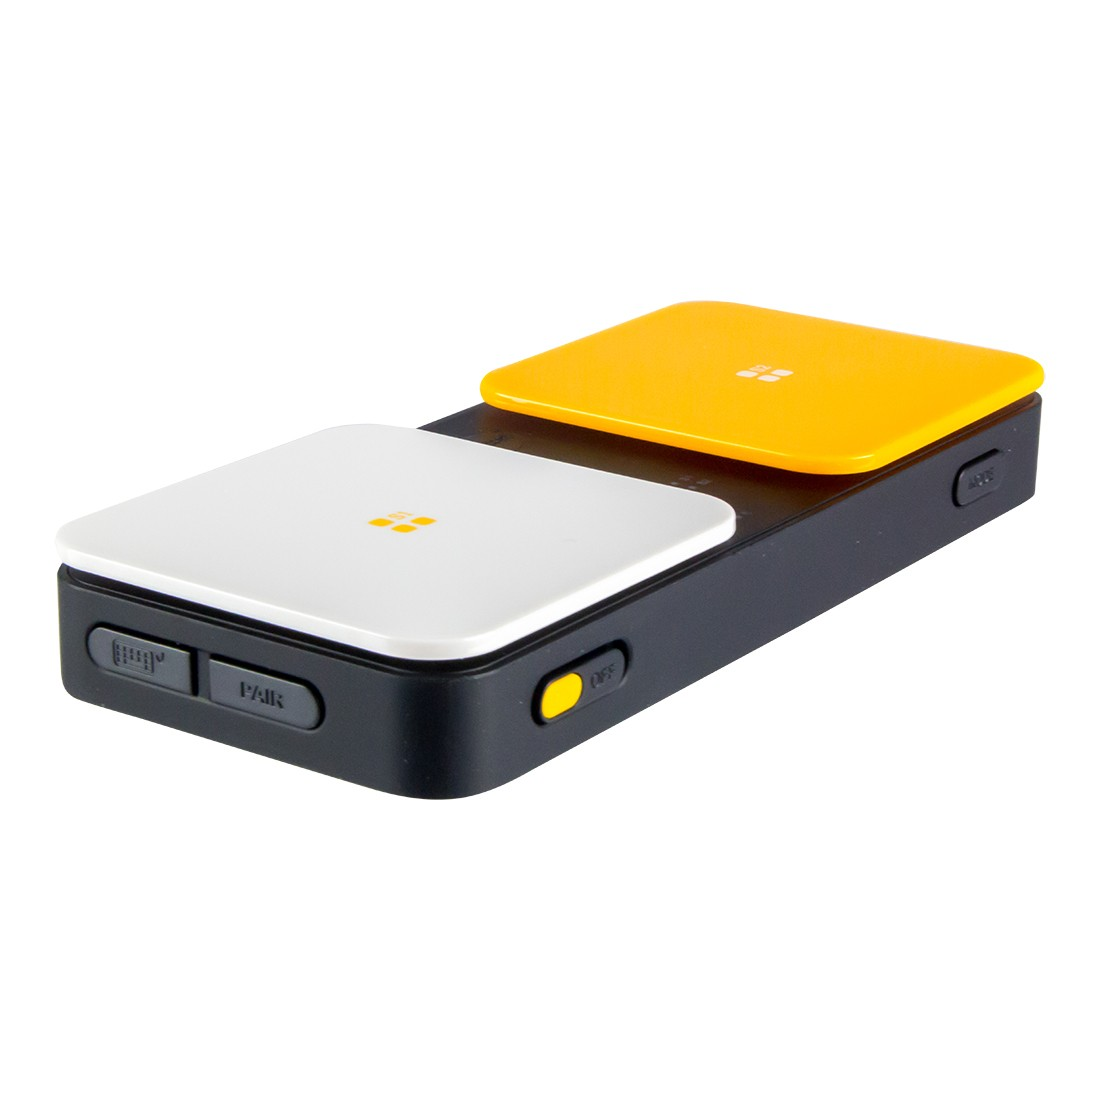
\includegraphics[width=.8\linewidth]{images/buttonsIPad.jpg}
  					\caption{\cite{ablenet:iPad}}
                    
				\end{subfigure}%
				\begin{subfigure}{.33\textwidth}
  					\centering
  					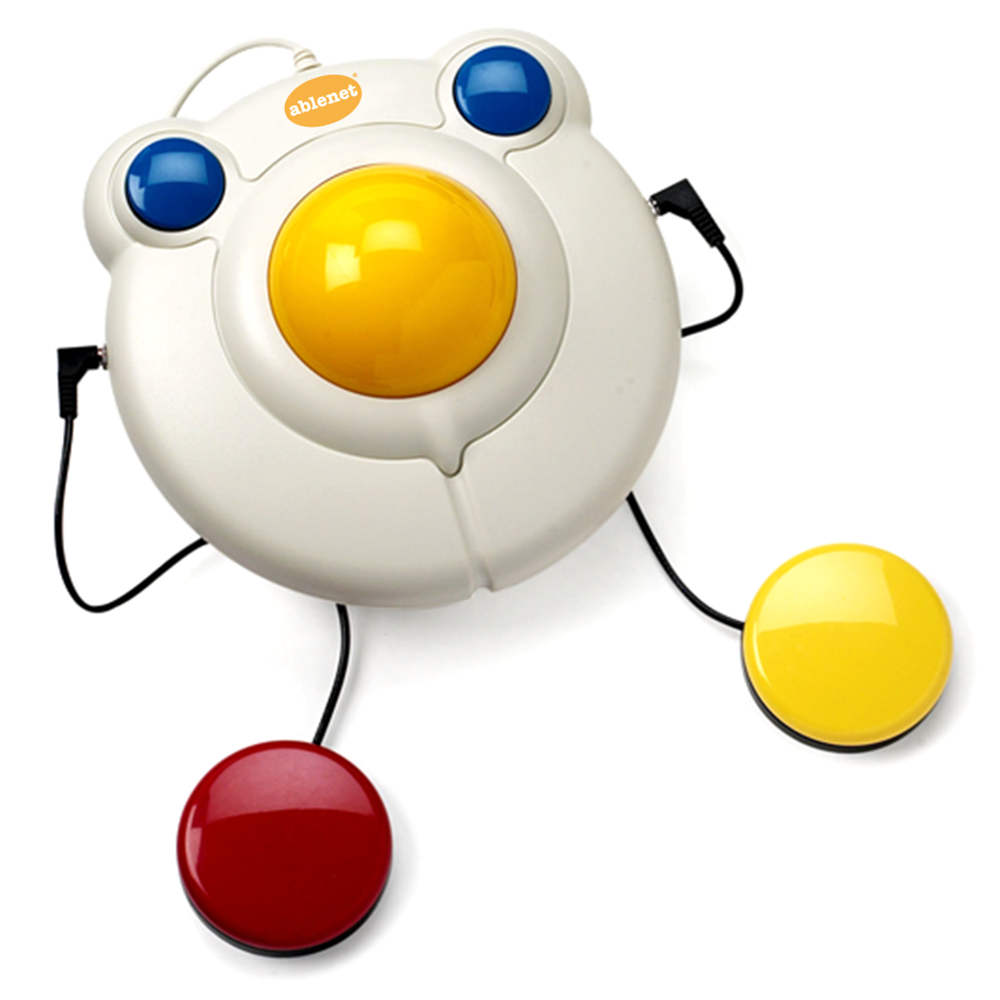
\includegraphics[width=.8\linewidth]{images/buttonsMouse.png}
  					\caption{\cite{ablenet:mouse}}
				\end{subfigure}
                \begin{subfigure}{.33\textwidth}
  					\centering
  					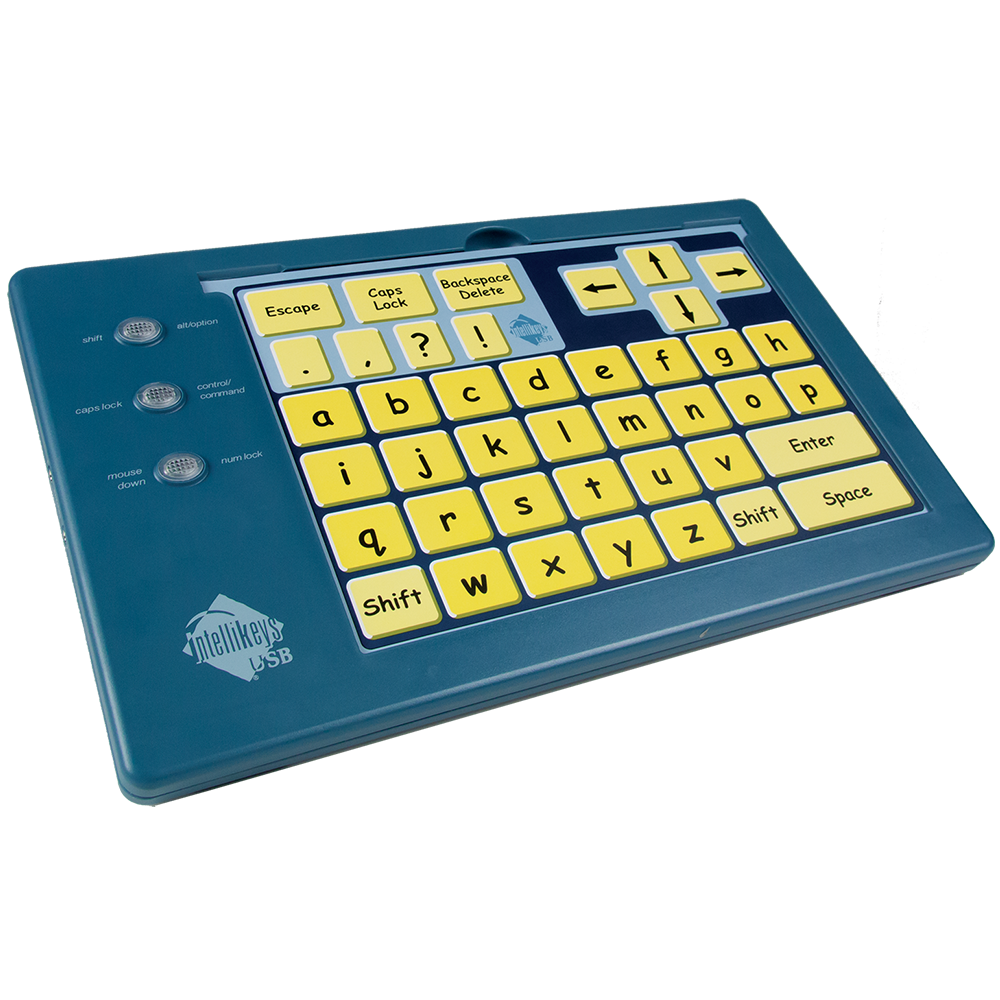
\includegraphics[width=.8\linewidth]{images/buttonsKeyboard.png}
  					\caption{\cite{ablenet:keyboard}}
				\end{subfigure}
                \caption{Taster mit mehreren Tasten von ablenet}
				\label{fig:ablenetMultipleButtons}
			\end{figure}
            

            
    \newpage
    \subsection{Sprachsoftware für Schwerstmehrfachbehinderte}
    
    -> Tobii Sonar Scribe
    -> andere Tobii ??
    -> andere Hersteller
    
    \subsection{Verwendung von Sprachsoftware im Schulalltag}
    
    Lehrer bereiten Wortschatz für kommende Unterichtstunde vor
    -> funktioiert gut
    -> spontane Unterhaltungen schwierig
    
	\subsection{Sprachsoftware in Unterhaltungs- und Massenelektronik}
    
    \newpage